\section{Square lattice}
\label{sec:square}

The case of the square lattice is extensively studied both at the mean field level and using \acs{QMC}.
Mean field results suggest that at half filling,  antiferromagnetic order persists even at weak coupling \cite{claveau_mean-field_2014, gouveia_magnetic_2015}, a result that we confirm with \acs{QMC}, reproducing the results of \cite{white_numerical_1989, hirsch_two-dimensional_1985}.

\begin{figure}[H]
\label{fig:mfHubbardPhaseDiagram}
\hspace{-0.18cm}
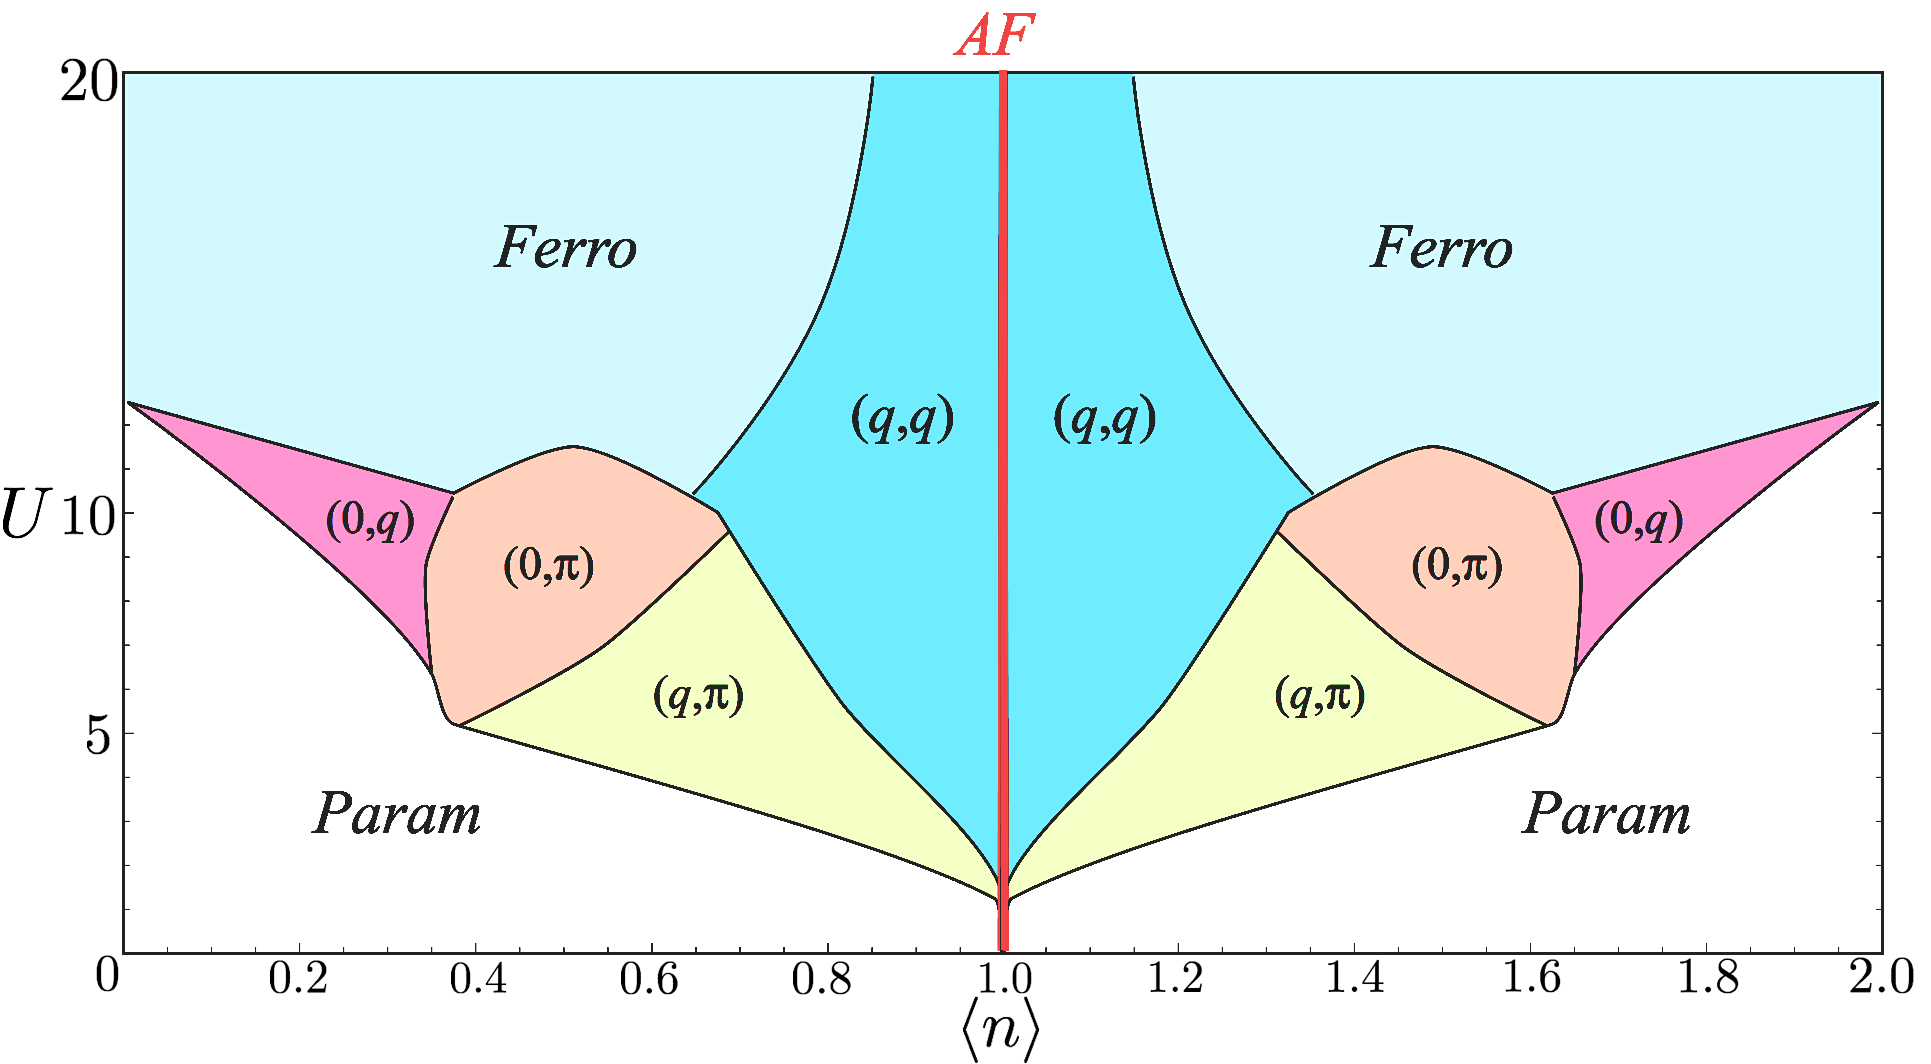
\includegraphics[scale=0.245]{Applications/mf-phase-diagram-hubbard}
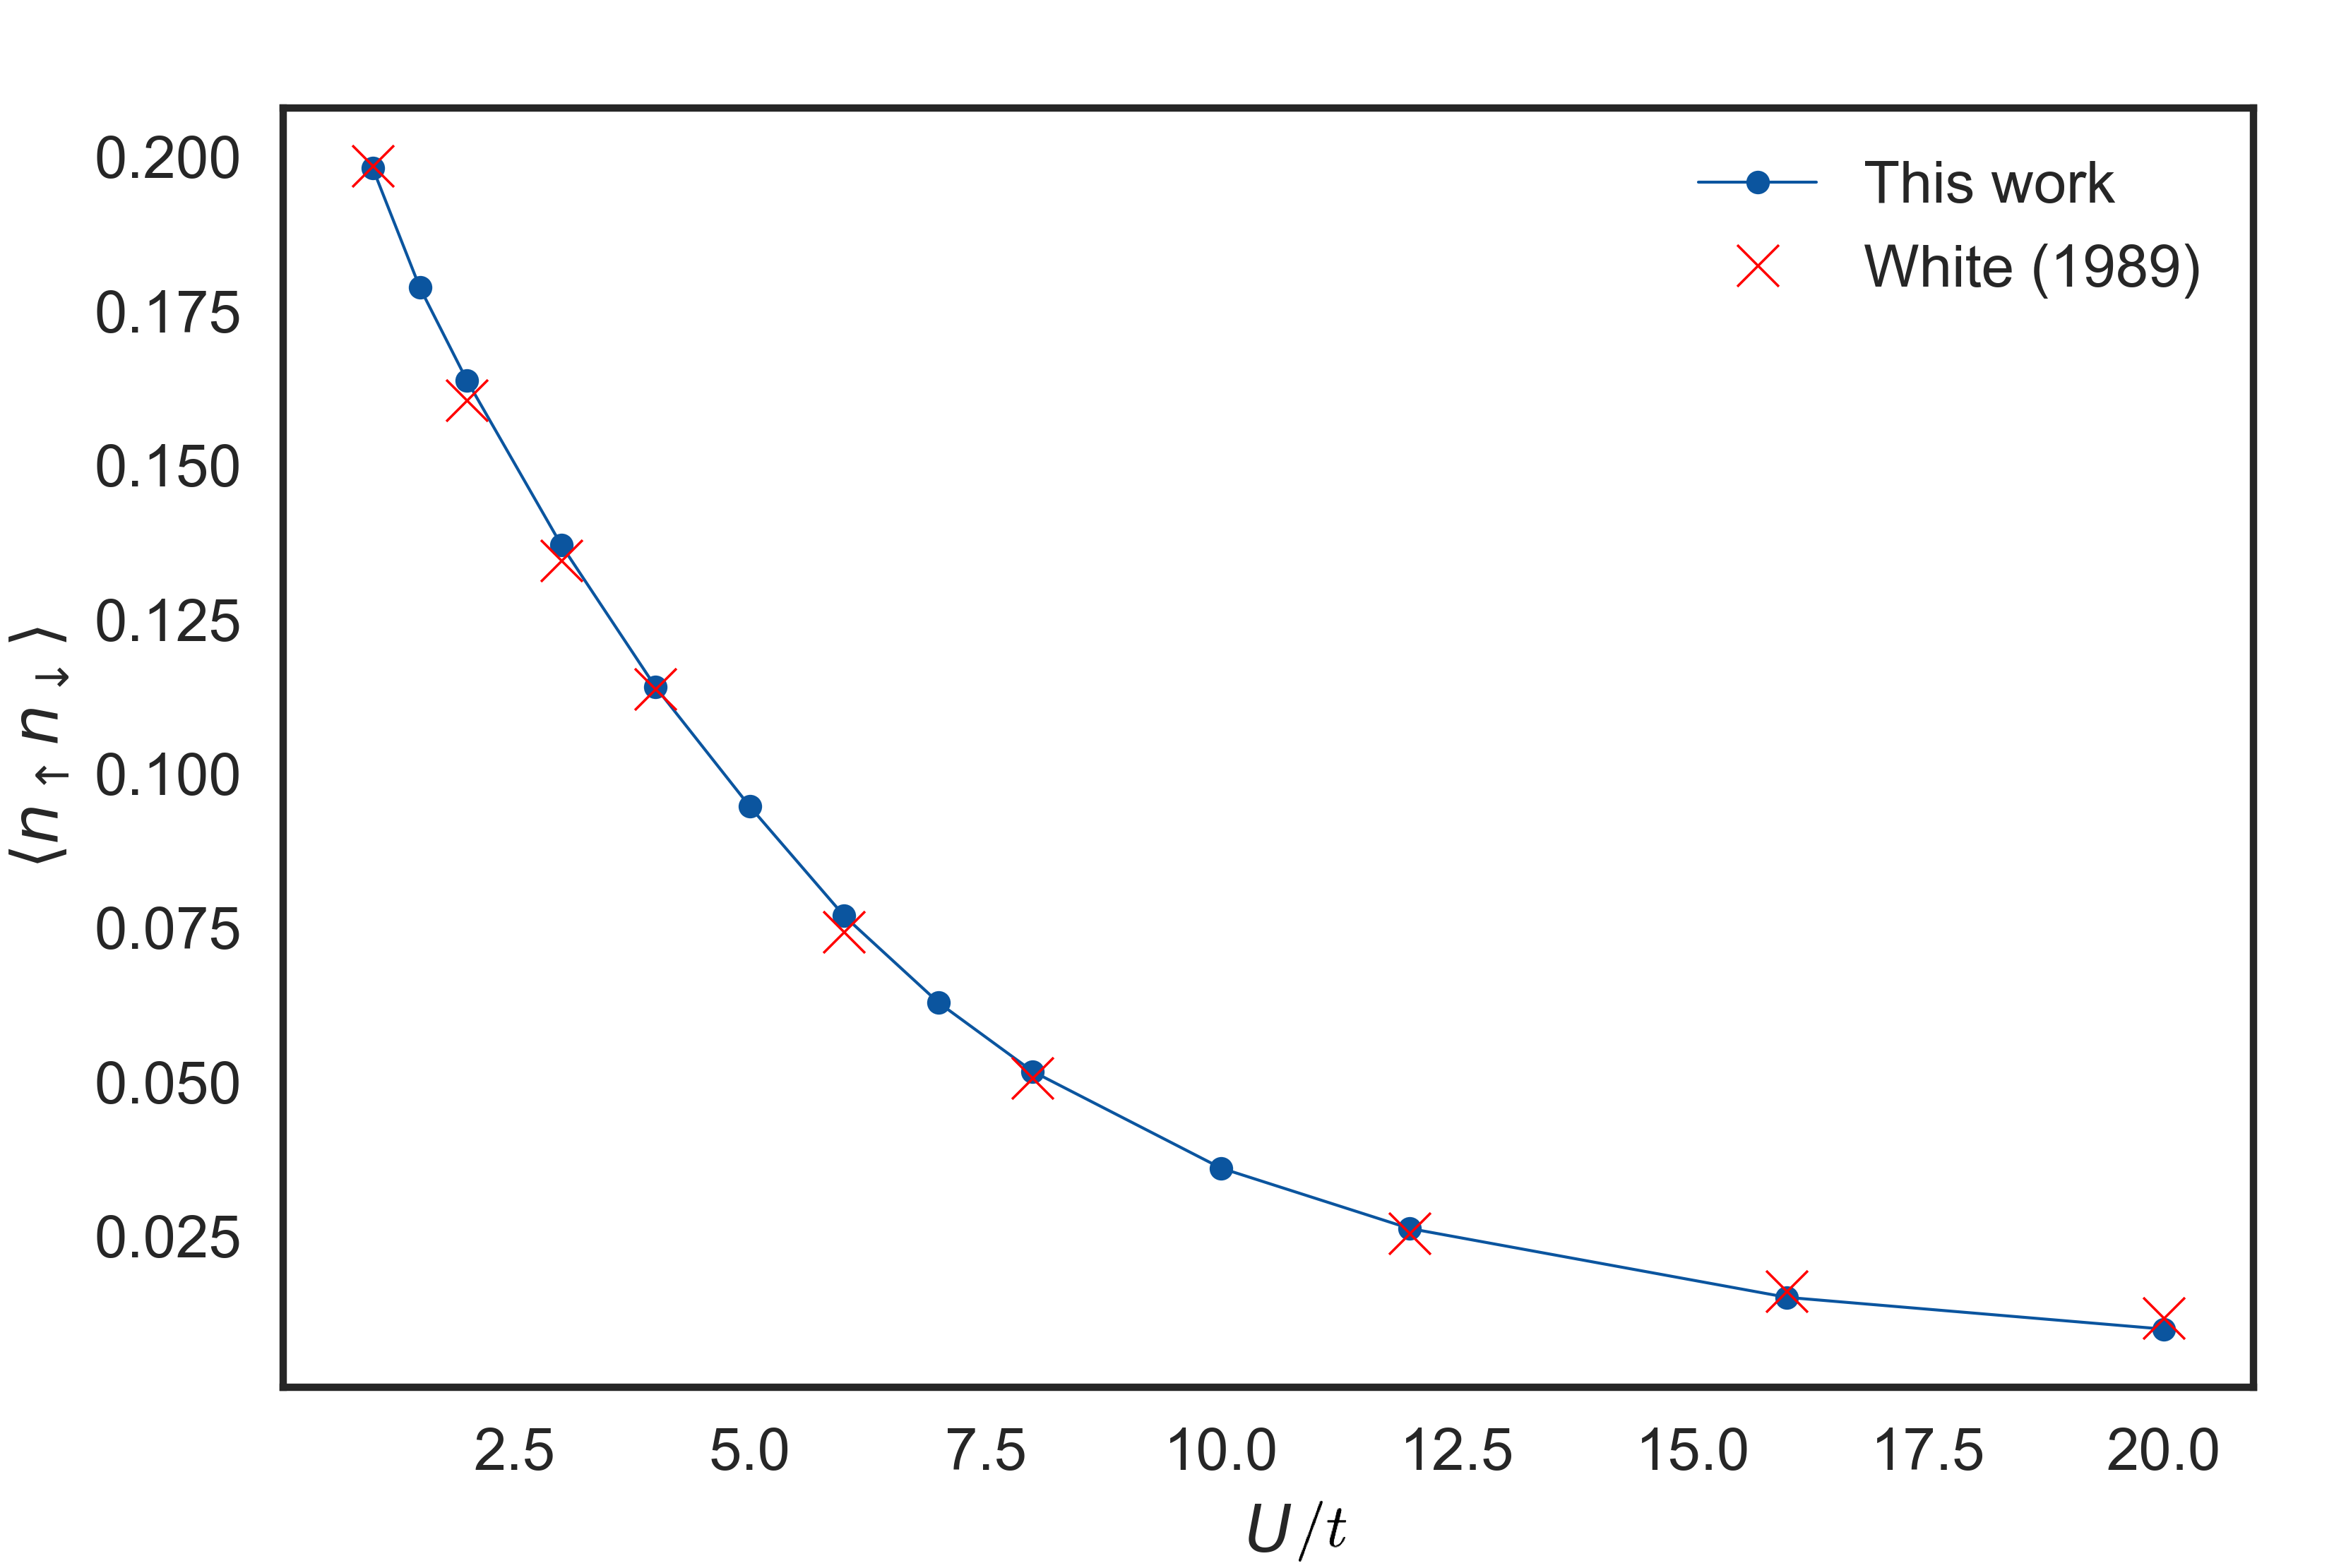
\includegraphics[scale=0.493]{Applications/square/nUpnDwSquare}
\caption[Mean field phase diagram of the Hubbard model. \ac{QMC} data showing the decrease of the double occupancy with increasing $U$.]{Left: Mean field phase diagram of the Hubbard model \cite{gouveia_magnetic_2015} (containing configurations with spiral order). Right: \ac{QMC} data showing the decrease of the double occupancy with increasing $U$.}
\end{figure}

\begin{figure}[H]\label{fig:corrSq}
\hspace{-0.3cm}
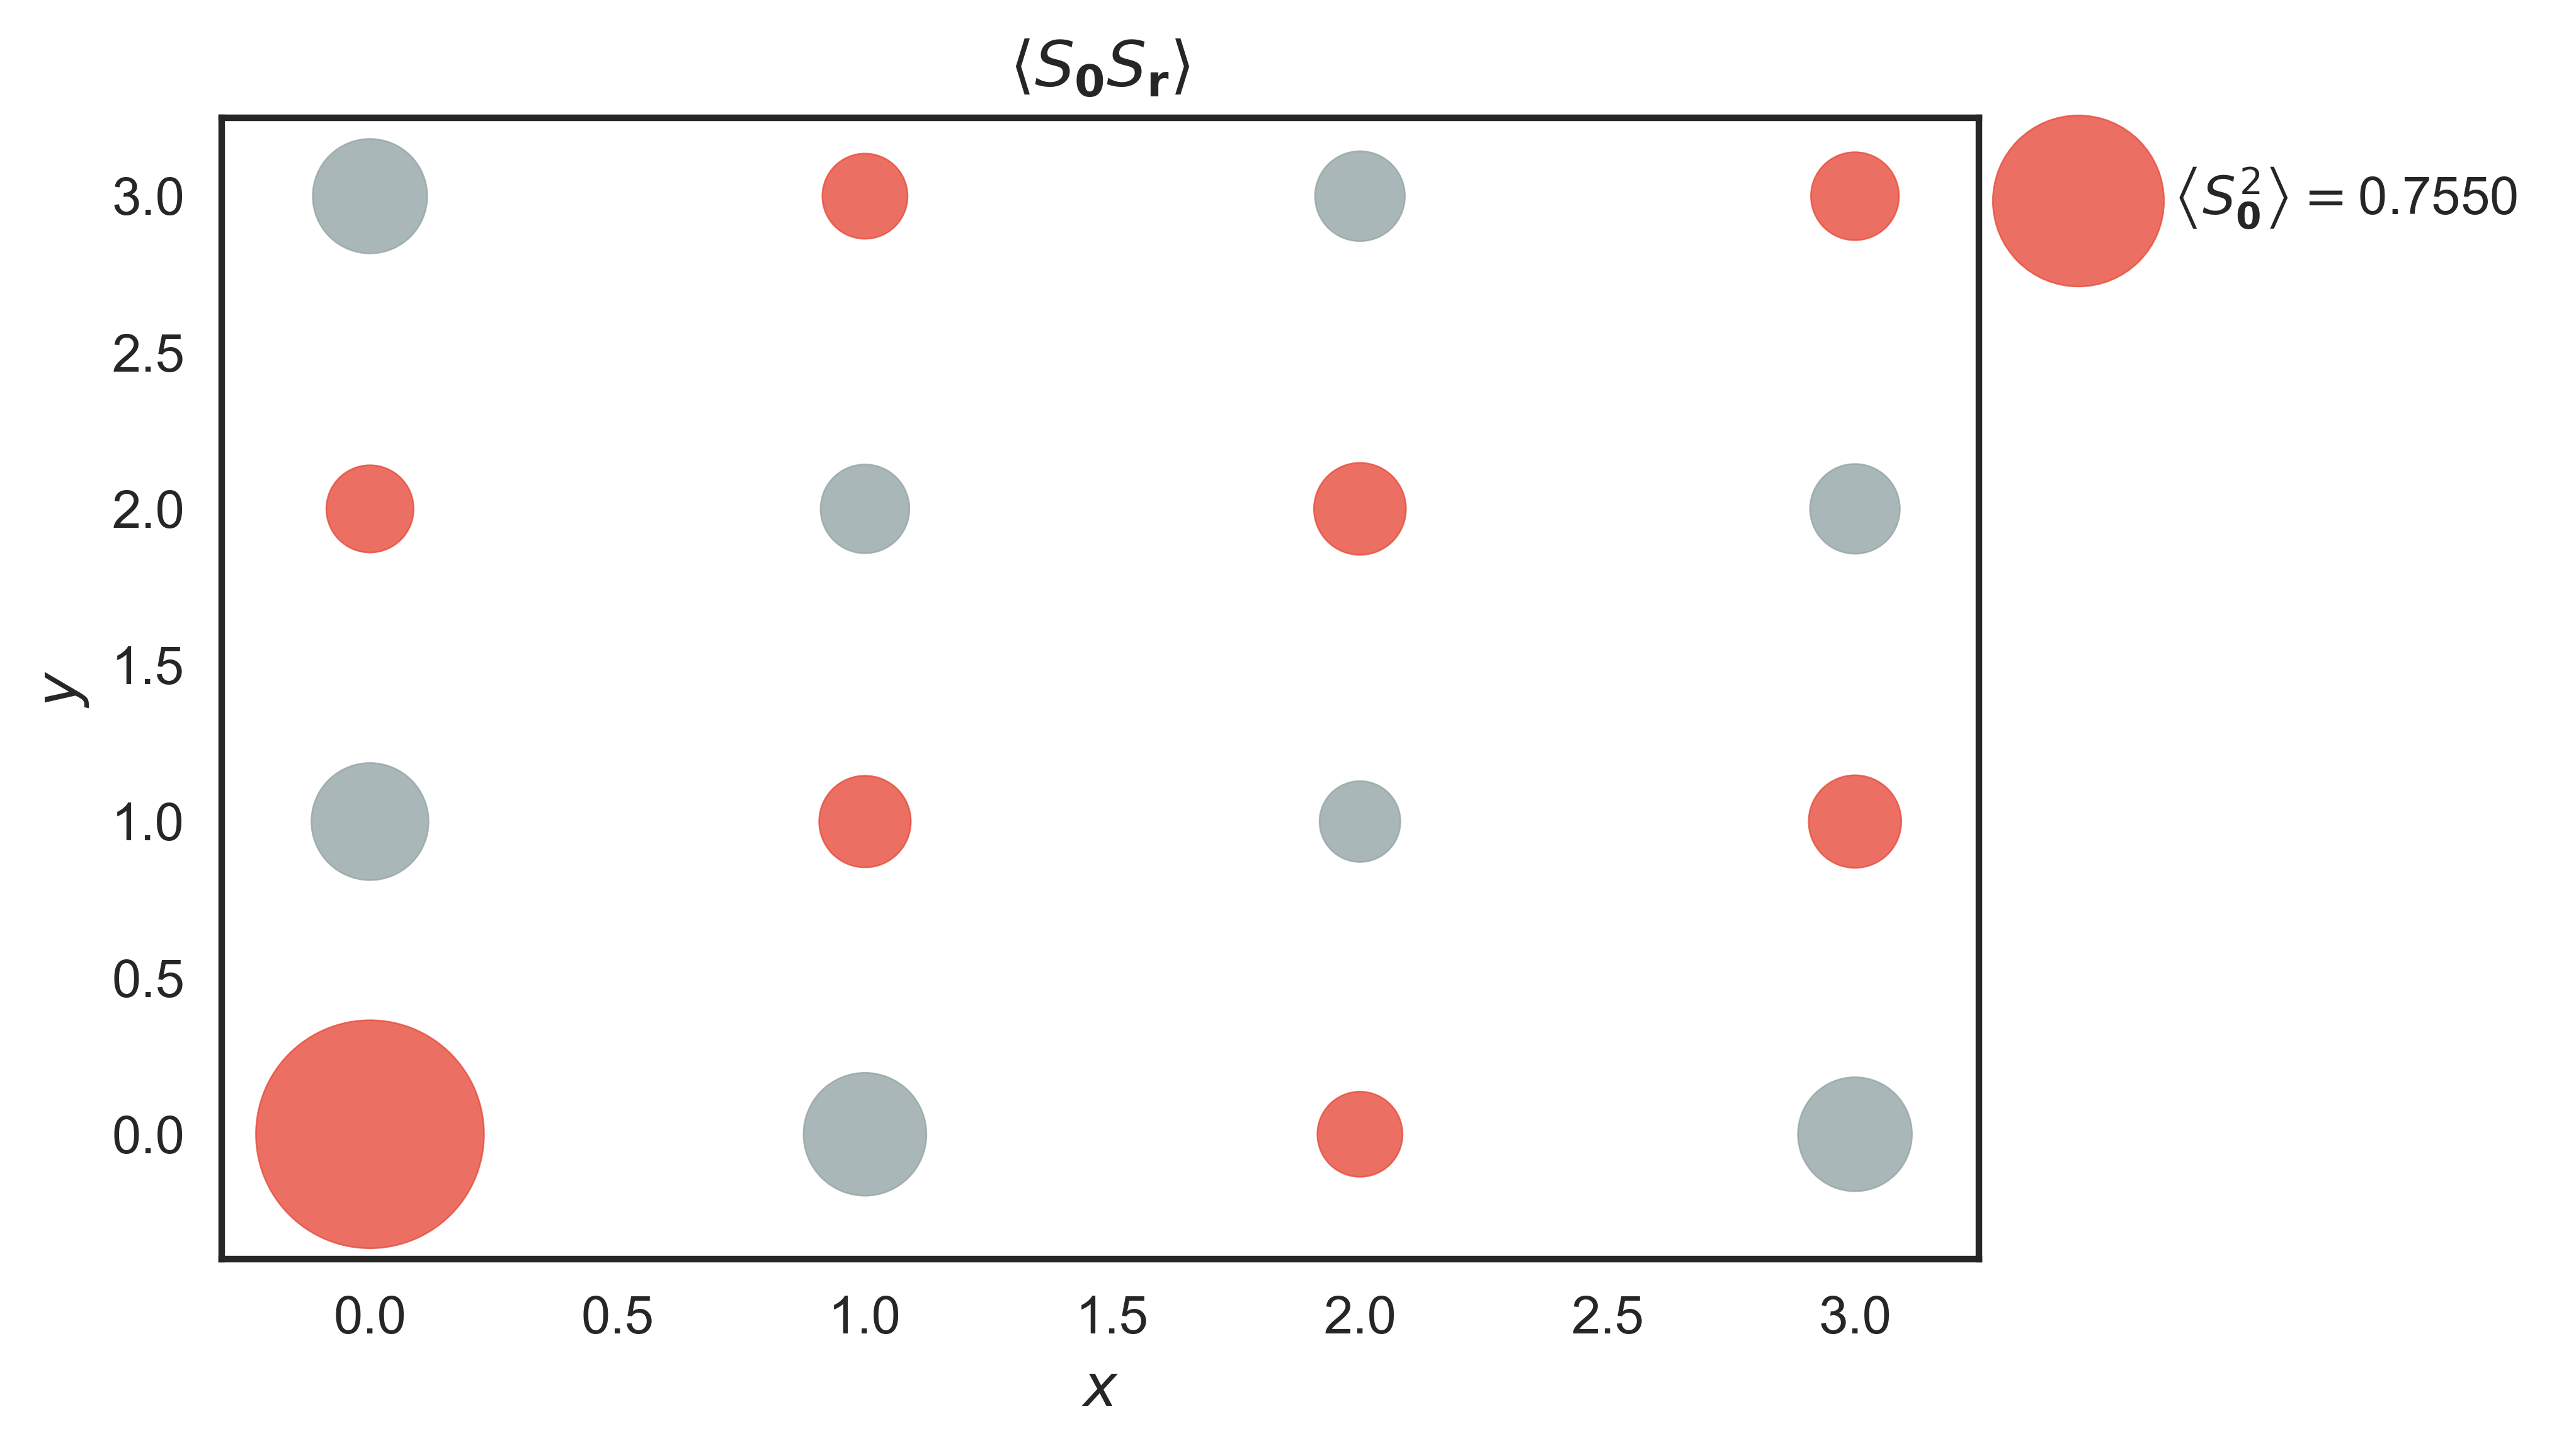
\includegraphics[scale=0.55]{Applications/square/CorrelationsDots}
\hspace{0.2cm}
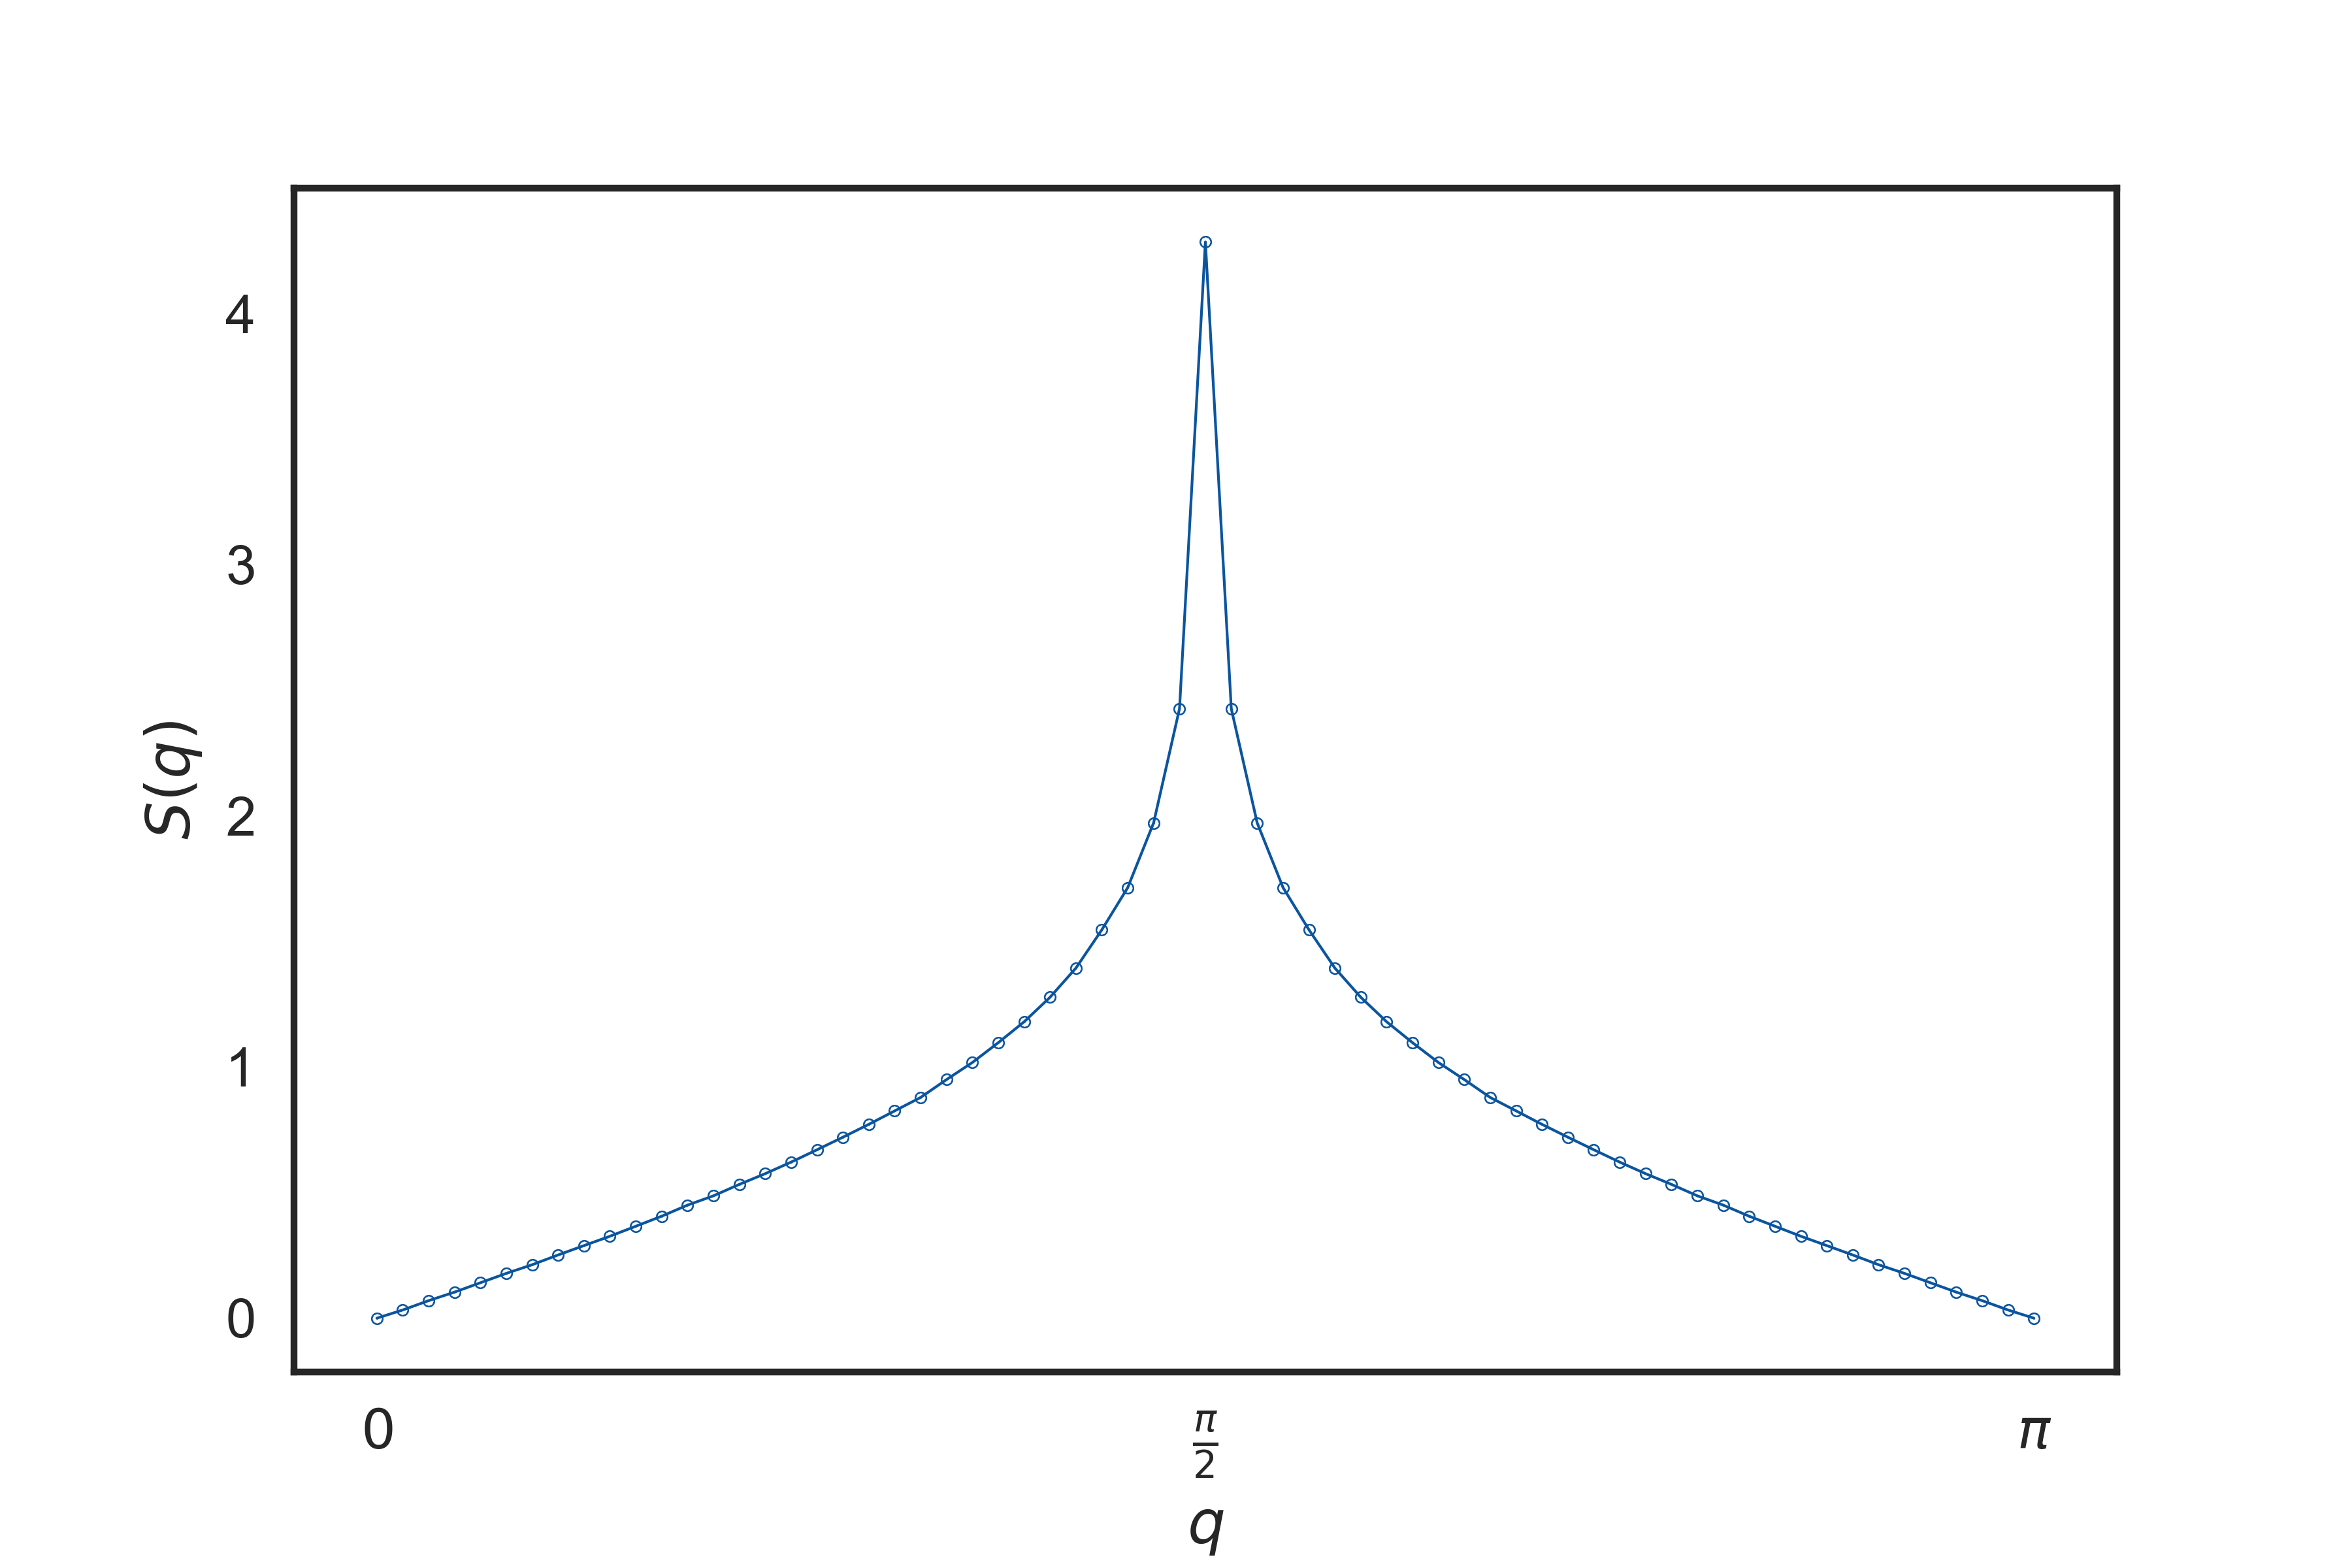
\includegraphics[scale=0.65]{Applications/square/S(q)}
\caption[Spin-spin correlations with respect to the point labeled $0$ on the lattice.
3D Plot of the magnetic structure factor]{Spin-spin correlations with respect to the point labeled $0$ on the lattice.}
\end{figure}

\begin{figure}[H]\label{fig:corrSq}
\hspace{-0.2cm}
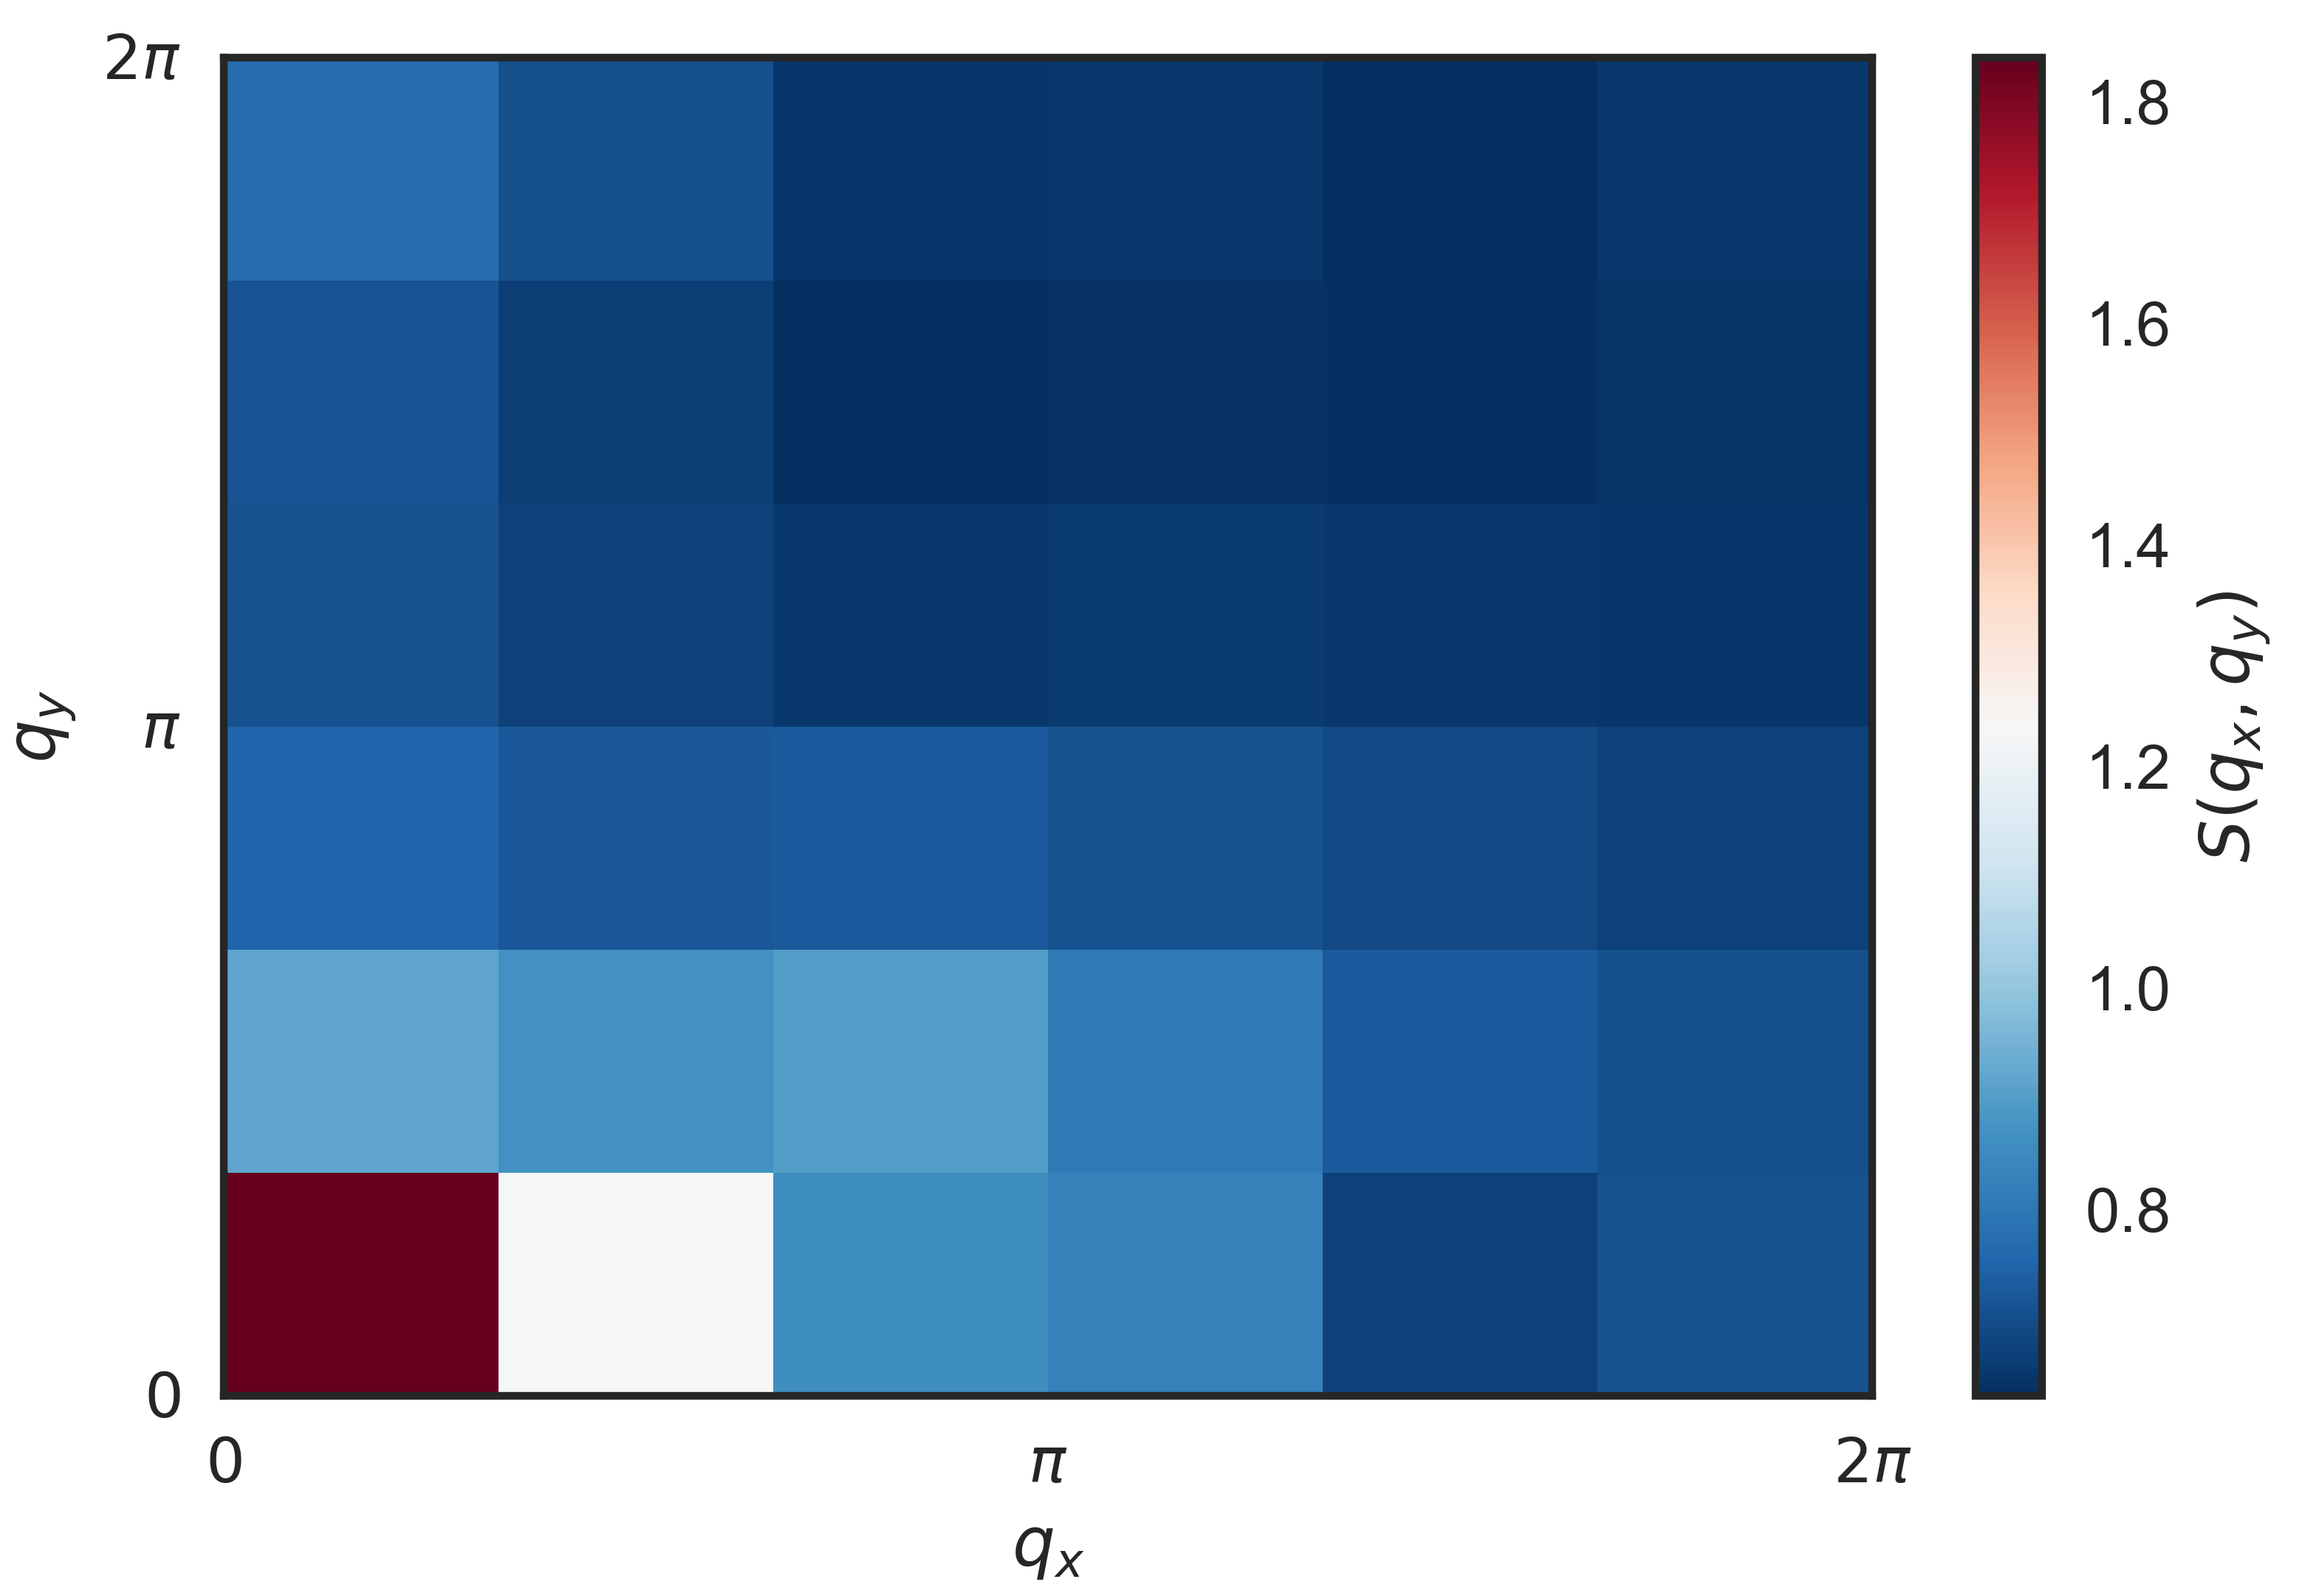
\includegraphics[scale=0.6]{Applications/square/S(q)pcolor.png}
\hspace{0.1cm}
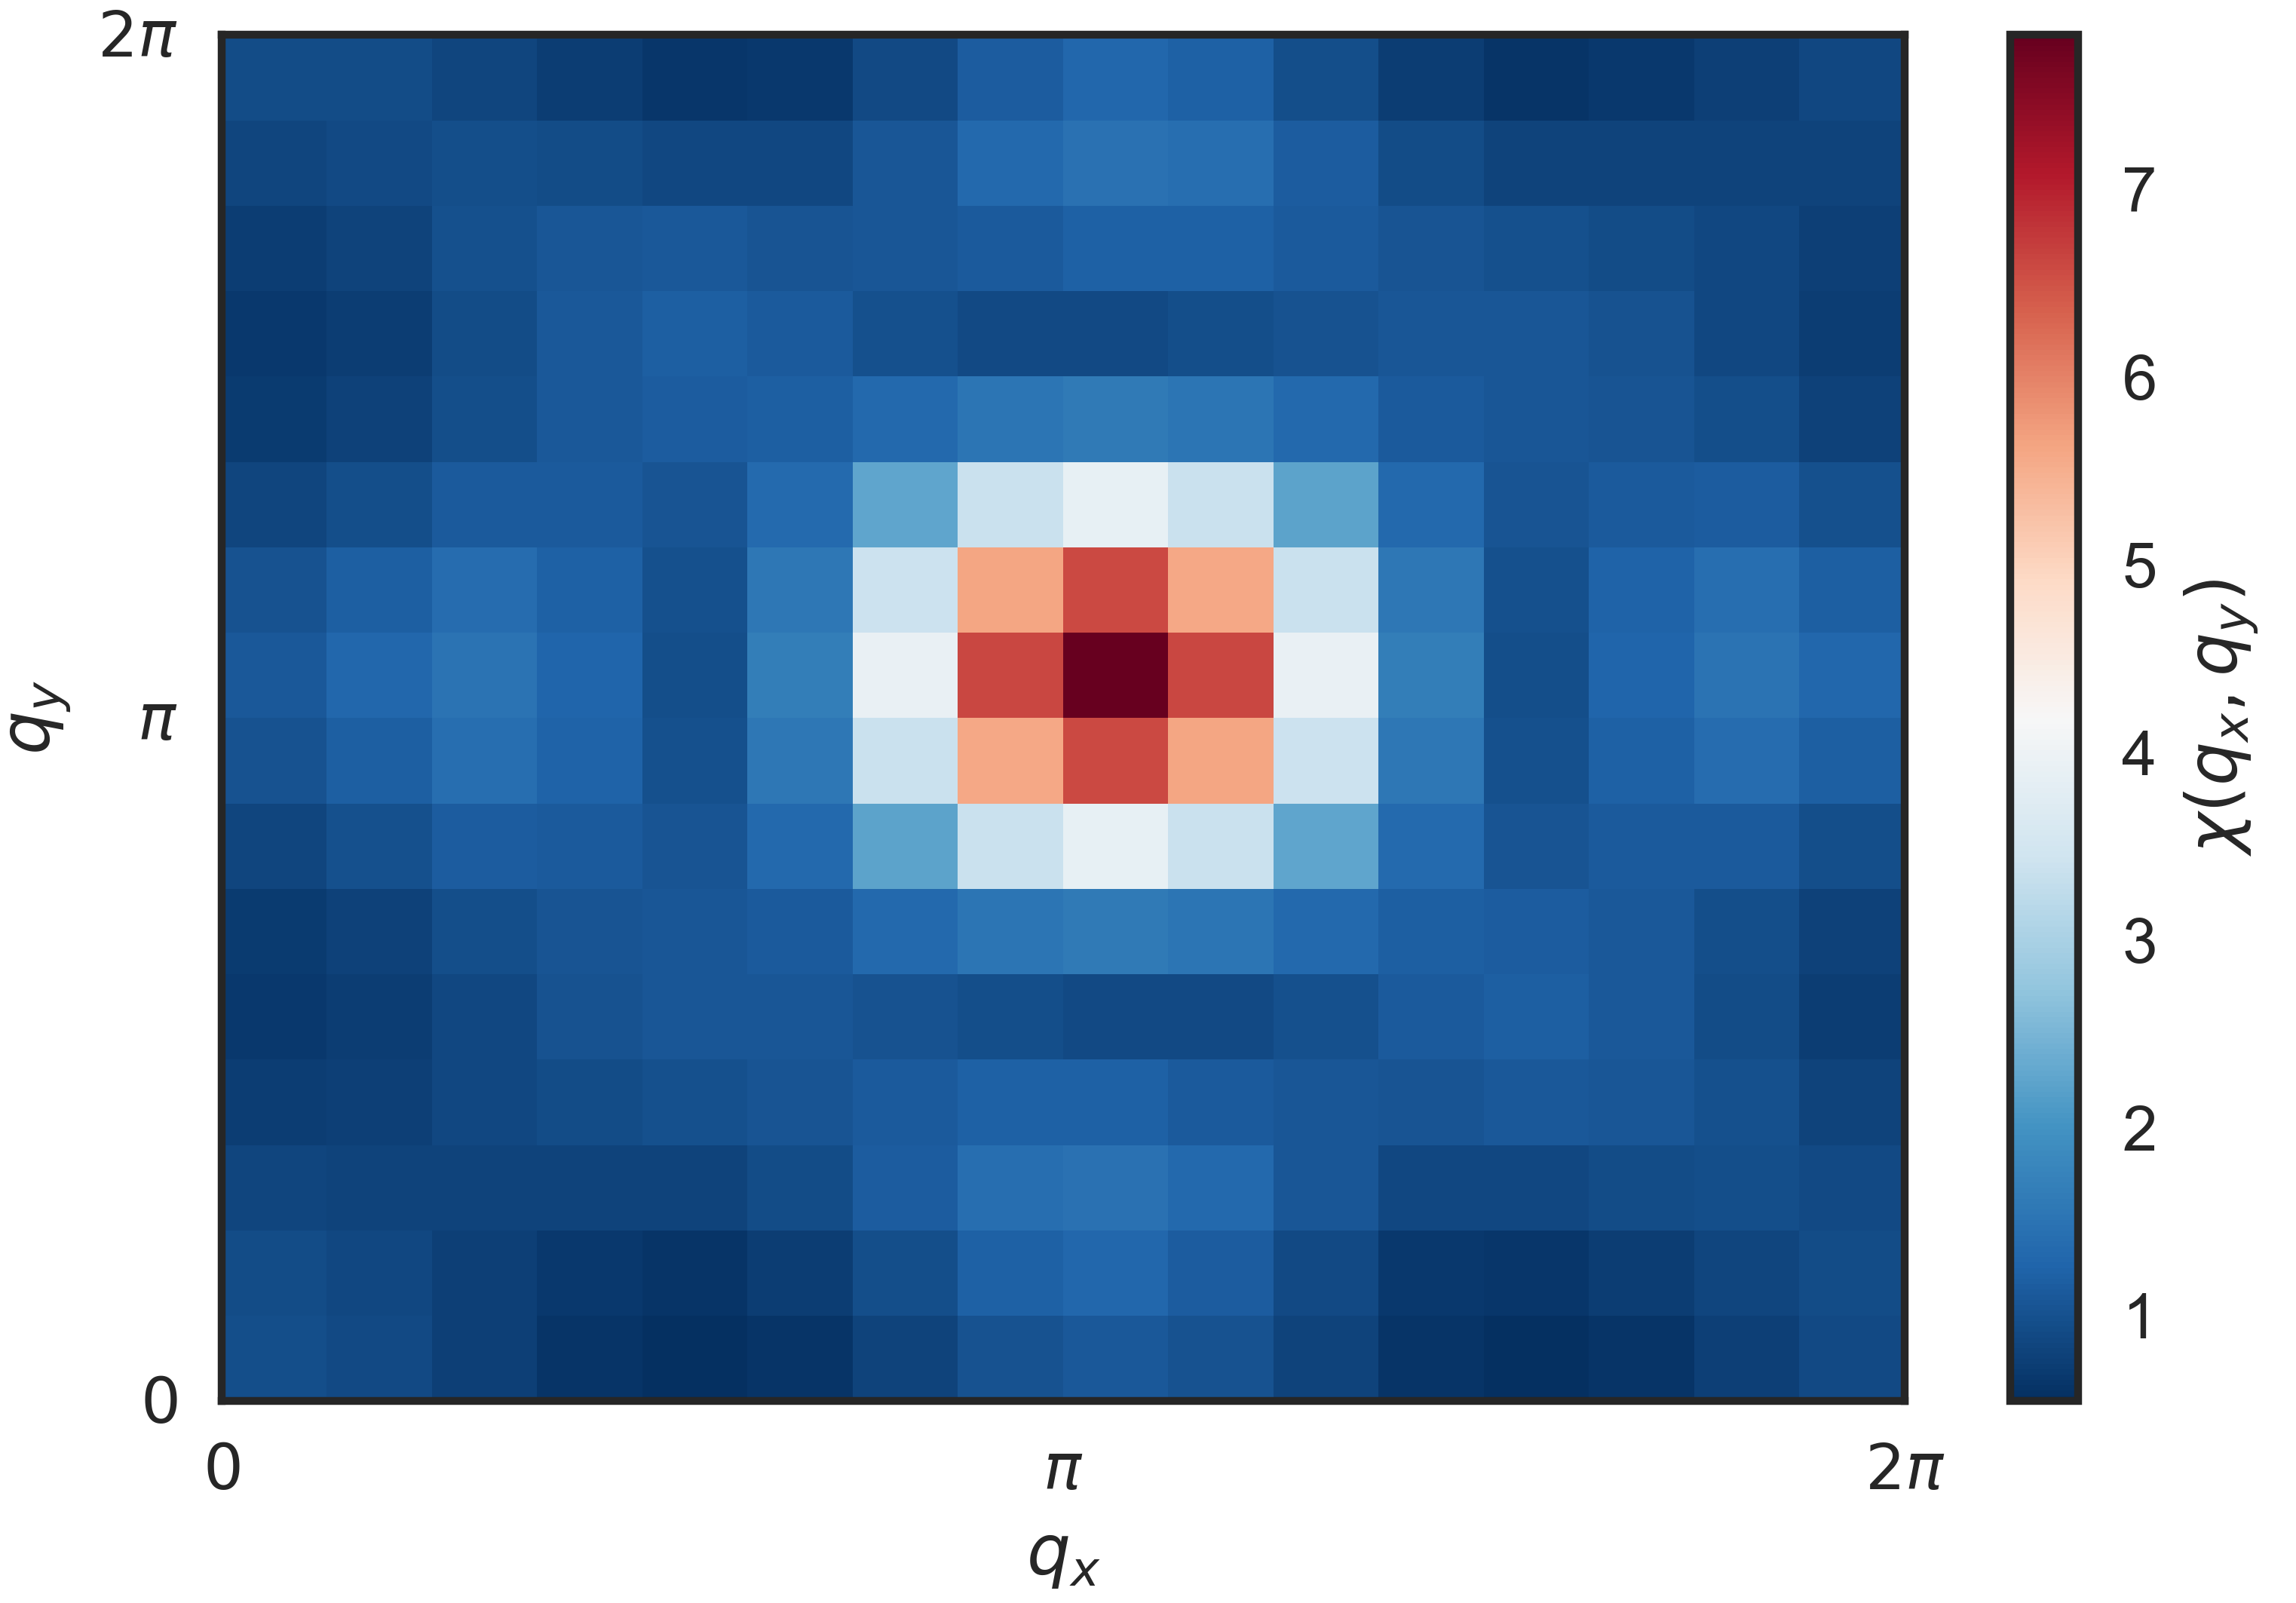
\includegraphics[scale=0.6]{Applications/square/chi(q)pcolor.png}
\caption[3D Plot of the magnetic structure factor]{3D Plot of the magnetic structure factor, showing a peak in $\bm \pi$.}
\end{figure}

\begin{figure}[H]\label{fig:corrSq}
\hspace{-0.4cm}
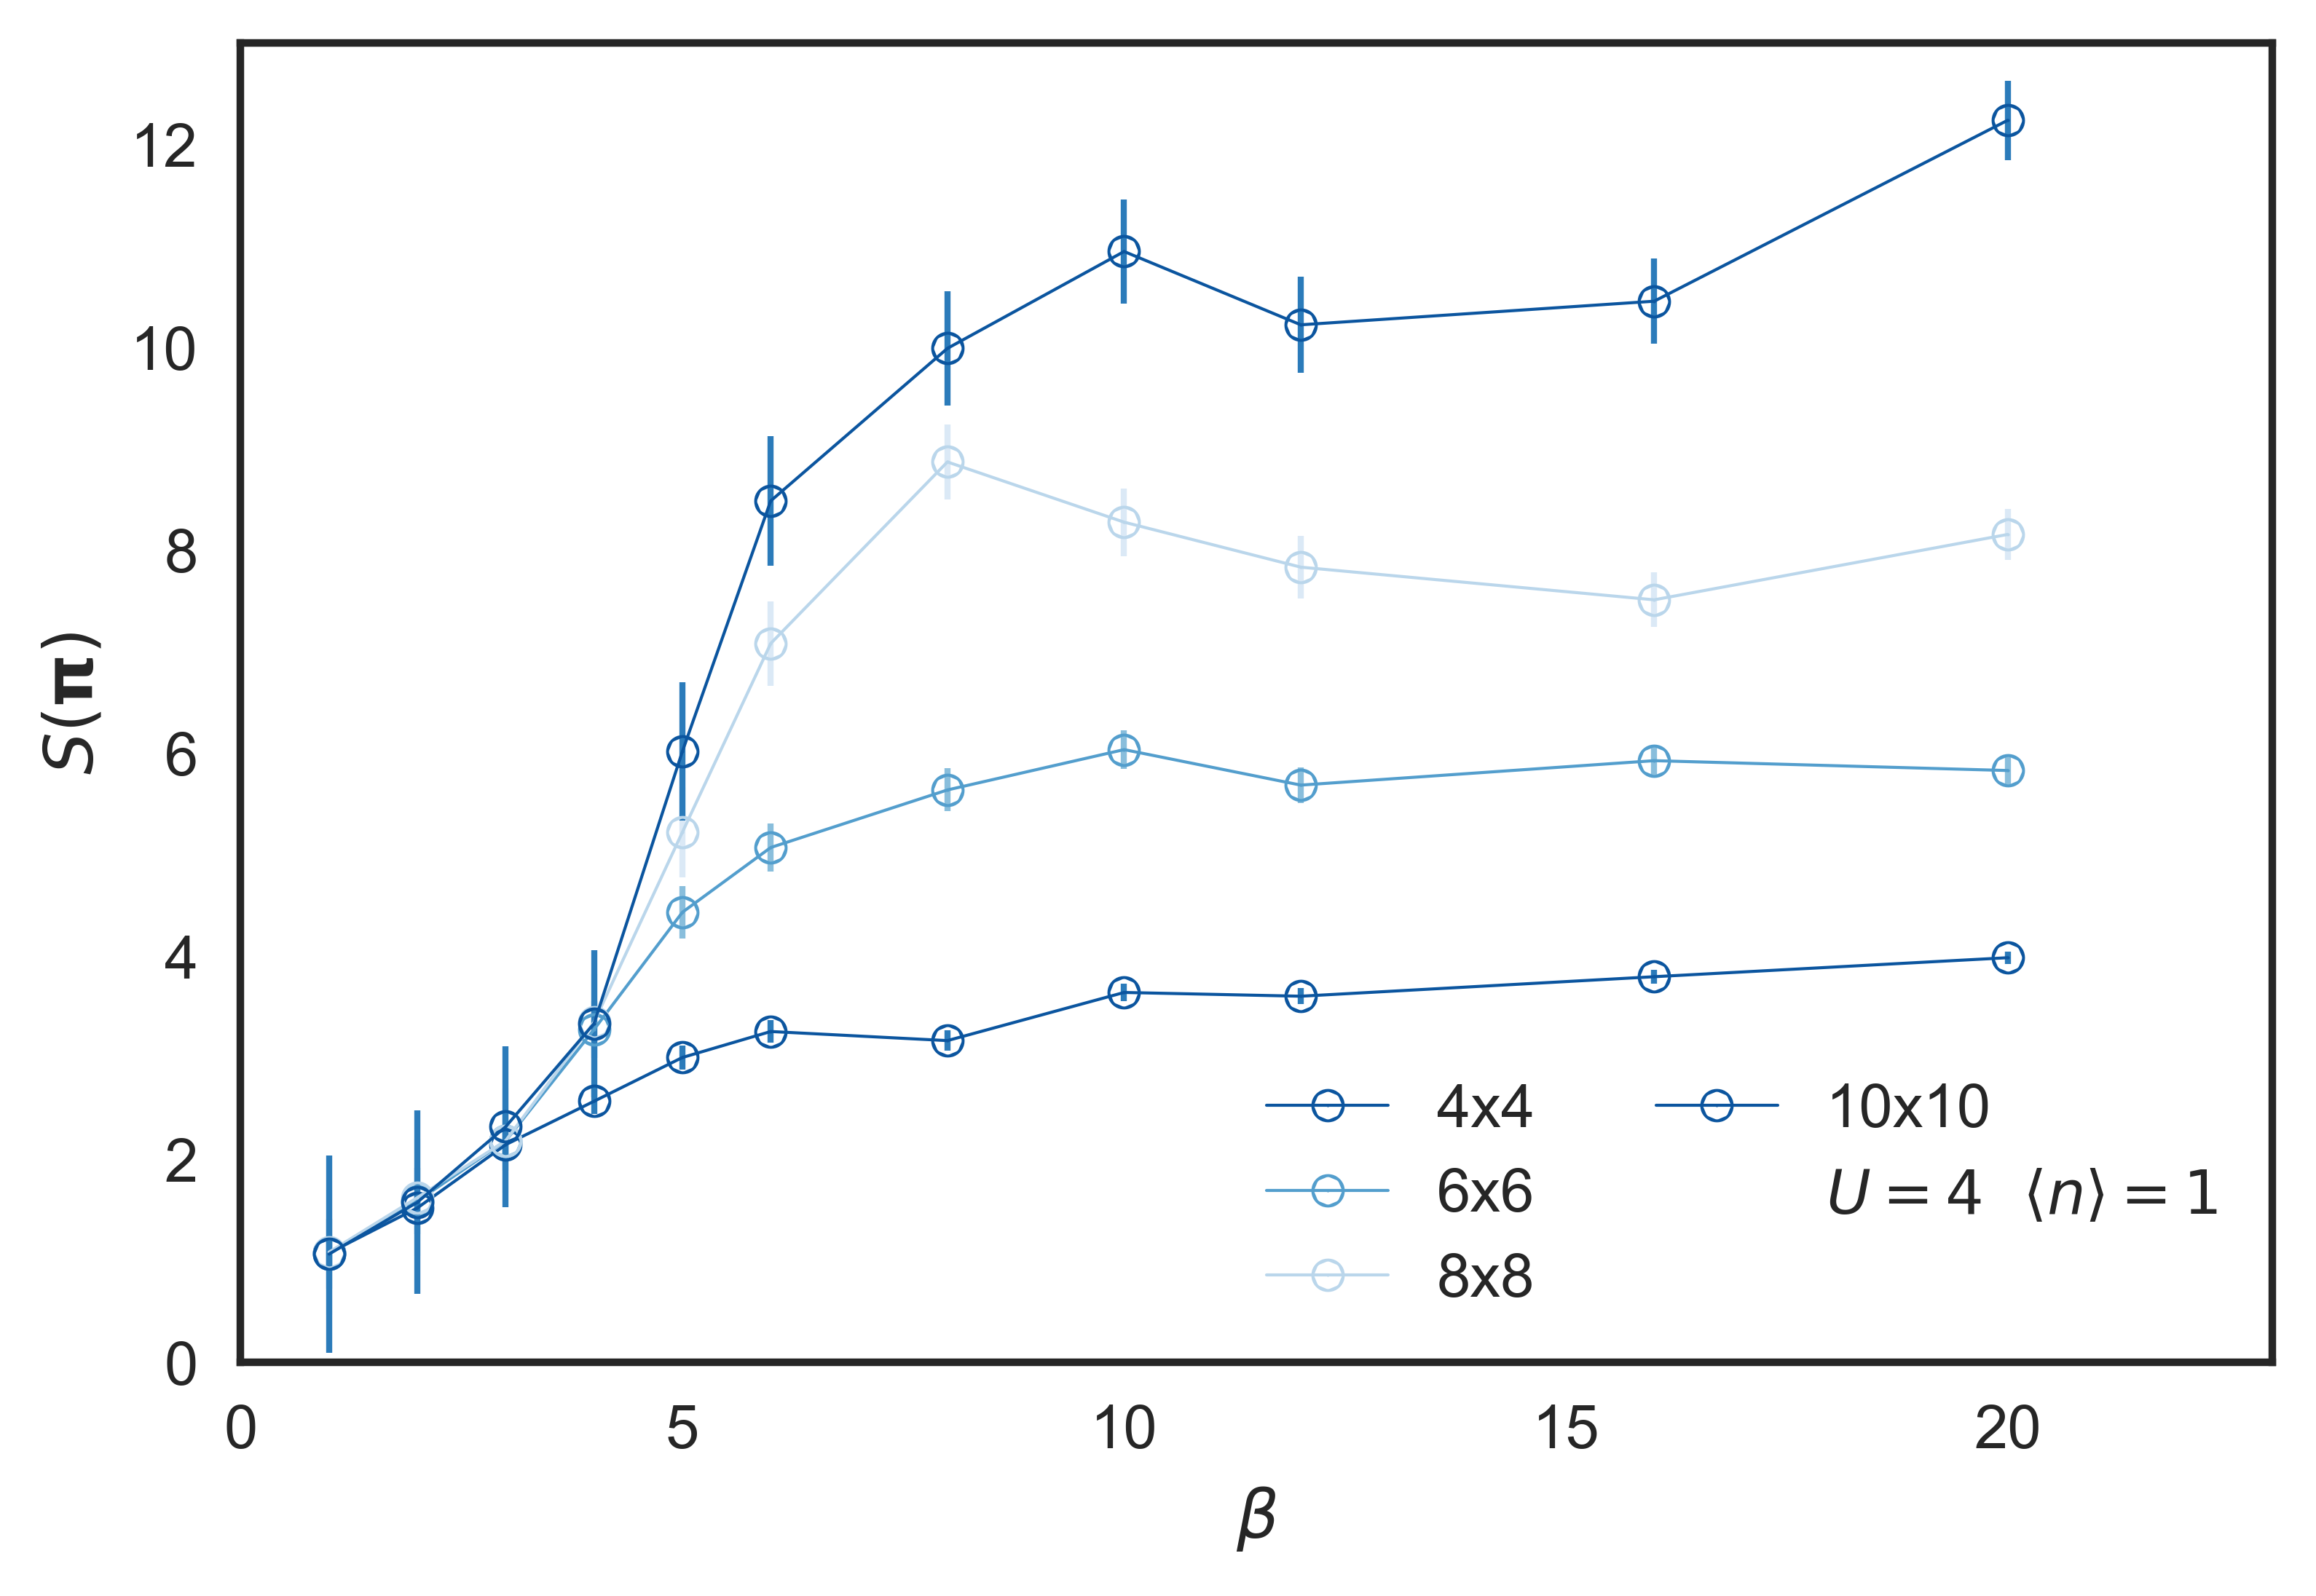
\includegraphics[scale=0.55]{Applications/square/Spipi.png}
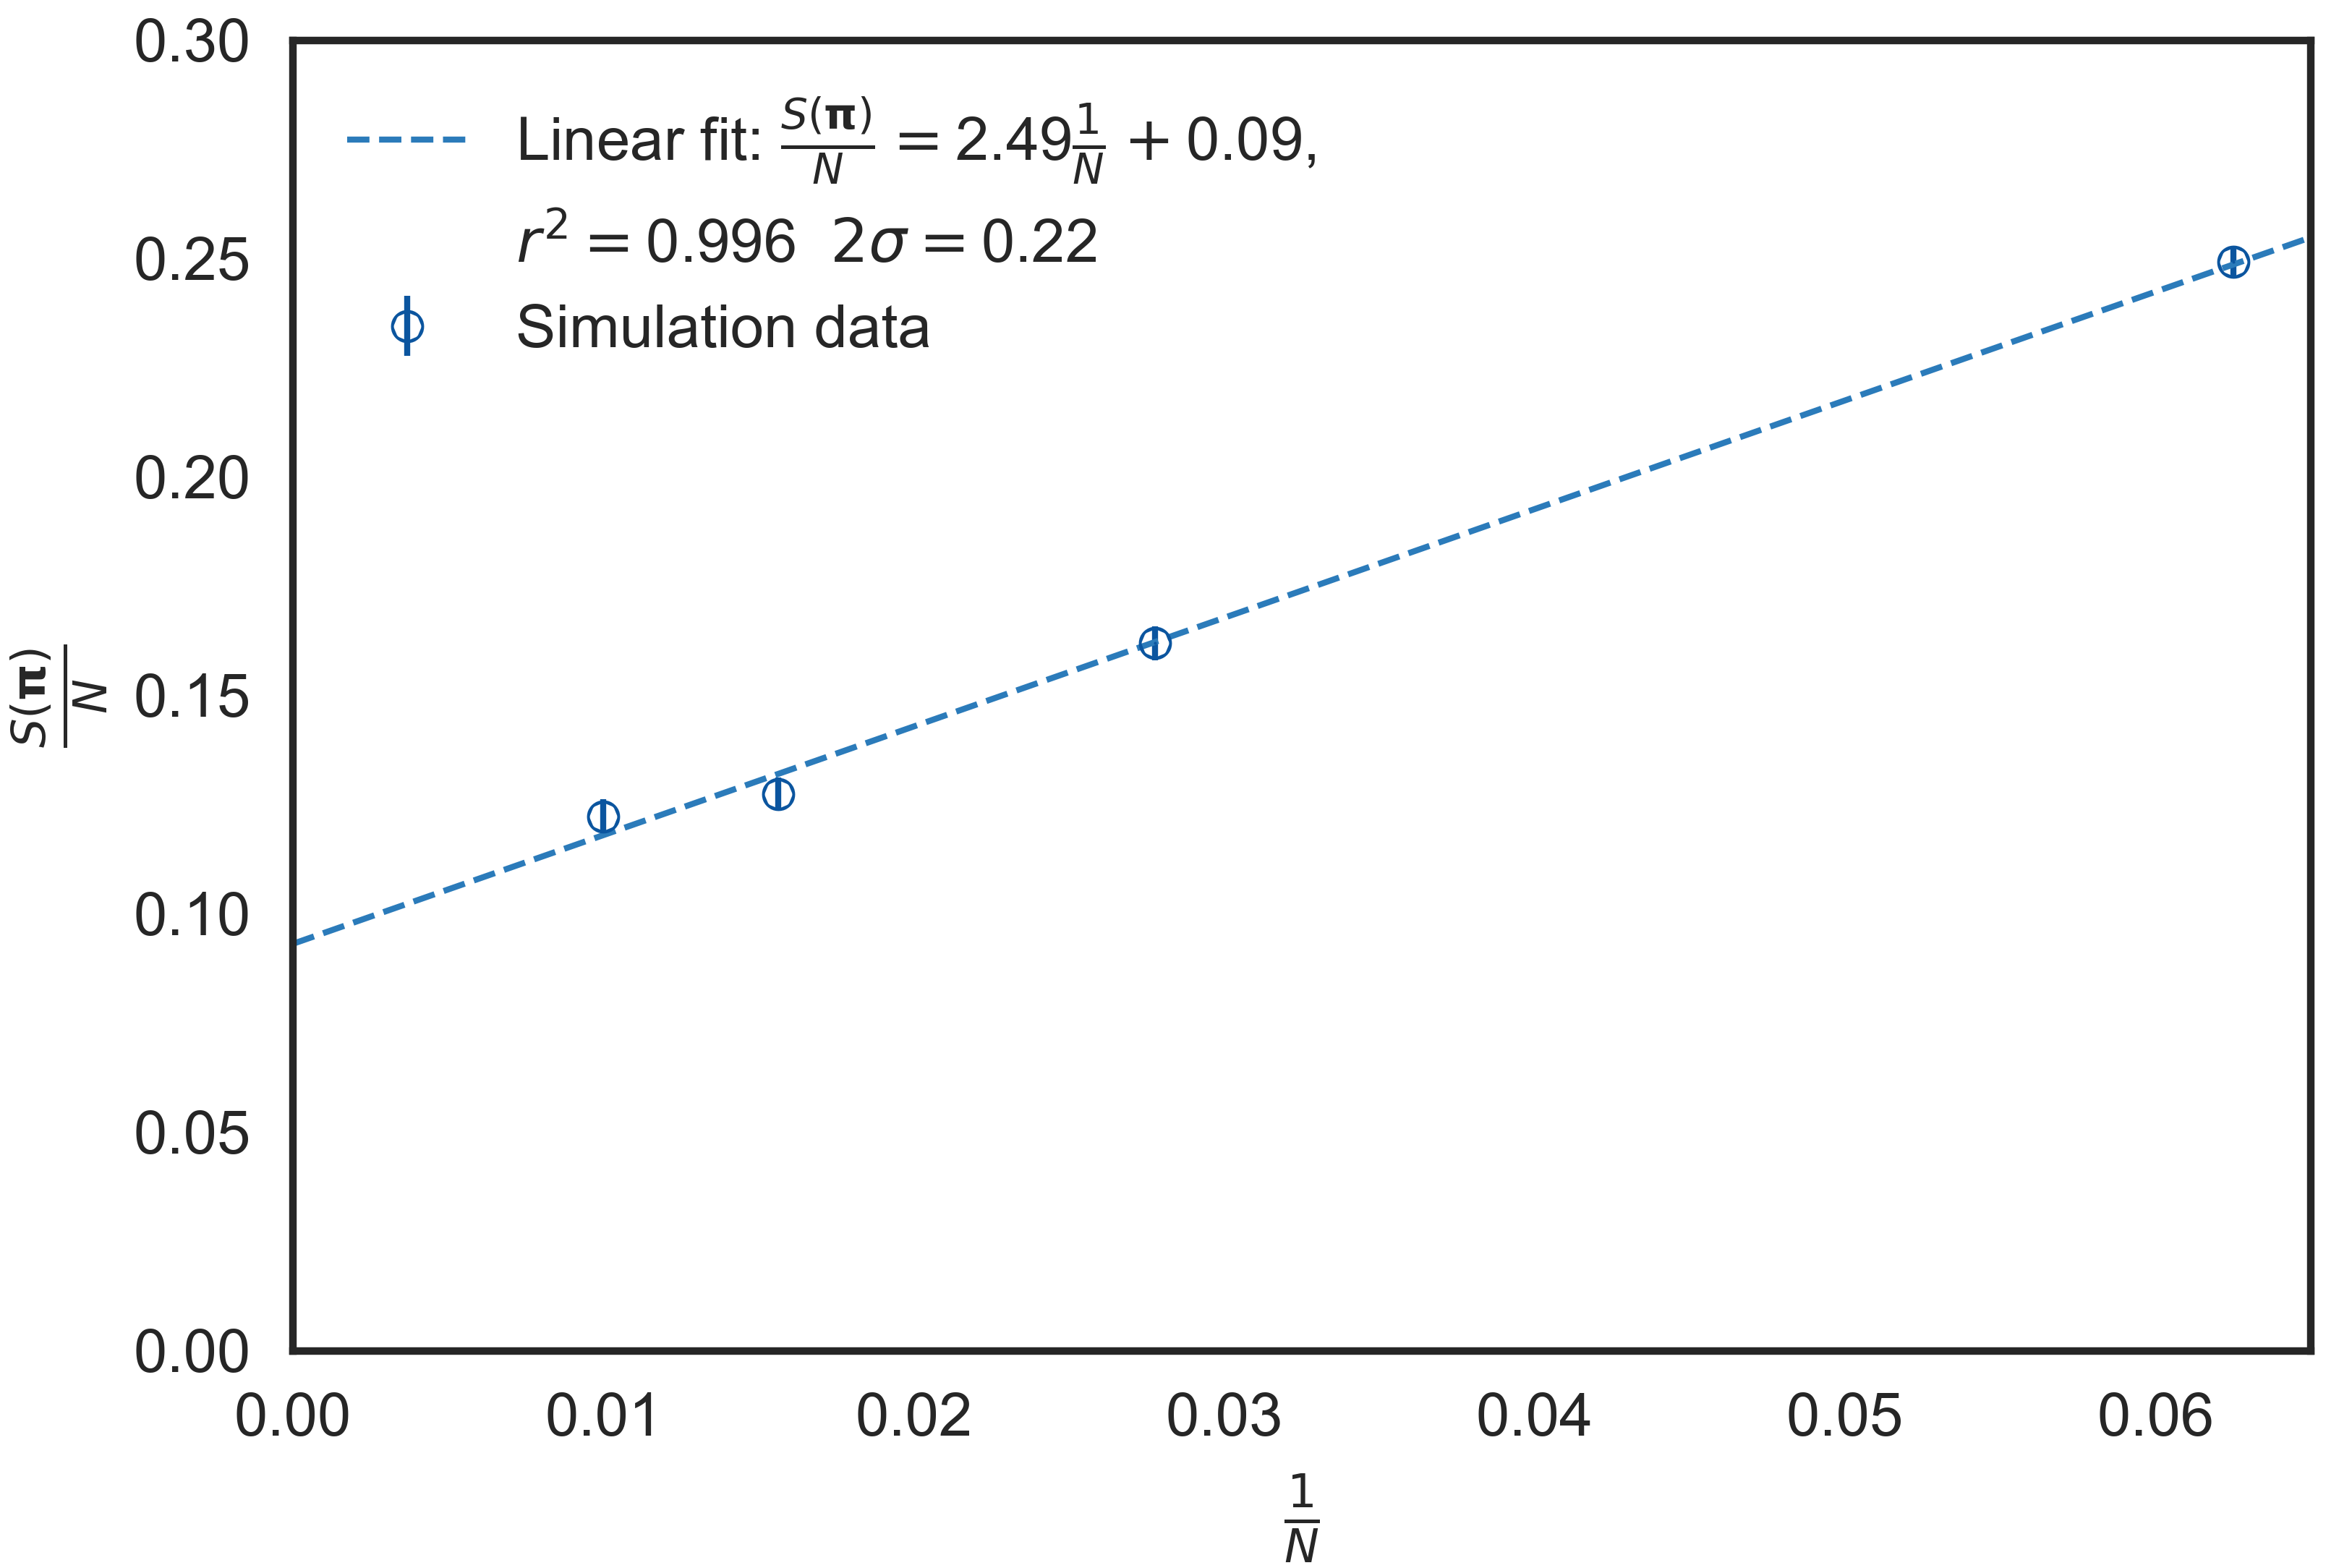
\includegraphics[scale=0.55]{Applications/square/extrapolationSpi.png}
\caption[]{}
\end{figure}